%%%%%%%%%%%%%%%%%%%%%%%%%%%%%%%%%%%%%%%%%%%%%%%%%%%%%%%%%%%%%%%%%%%%%%
% WWW 2027 공식 LaTeX 템플릿 (Murfy 제공)
% Official author kit: ACM acmart (acmart.cls + sample-sigconf)
% The ACM Web Conference. Research track: 익명 제출, OpenReview. Full paper 마감 2026-10-25 (Abstract 10-18)
% 킷 확인일: 2026-08-28 · 대상 회차: WWW 2027
%%%%%%%%%%%%%%%%%%%%%%%%%%%%%%%%%%%%%%%%%%%%%%%%%%%%%%%%%%%%%%%%%%%%%%
%%
%% This is file `sample-sigconf.tex',
%% generated with the docstrip utility.
%%
%% The original source files were:
%%
%% samples.dtx  (with options: `all,proceedings,bibtex,sigconf')
%% 
%% IMPORTANT NOTICE:
%% 
%% For the copyright see the source file.
%% 
%% Any modified versions of this file must be renamed
%% with new filenames distinct from sample-sigconf.tex.
%% 
%% For distribution of the original source see the terms
%% for copying and modification in the file samples.dtx.
%% 
%% This generated file may be distributed as long as the
%% original source files, as listed above, are part of the
%% same distribution. (The sources need not necessarily be
%% in the same archive or directory.)
%%
%%
%% Commands for TeXCount
%TC:macro \cite [option:text,text]
%TC:macro \citep [option:text,text]
%TC:macro \citet [option:text,text]
%TC:envir table 0 1
%TC:envir table* 0 1
%TC:envir tabular [ignore] word
%TC:envir displaymath 0 word
%TC:envir math 0 word
%TC:envir comment 0 0
%%
%% The first command in your LaTeX source must be the \documentclass
%% command.
%%
%% For submission and review of your manuscript please change the
%% command to \documentclass[manuscript, screen, review]{acmart}.
%%
%% When submitting camera ready or to TAPS, please change the command
%% to \documentclass[sigconf]{acmart} or whichever template is required
%% for your publication.
%%
%%
% WWW 2027 short paper: 4 pages including references, double-blind review.
% Remove "anonymous" to preview the author block (kept below in the source).
\documentclass[sigconf,anonymous,review]{templates/acmart}
% ACM first-page classification and citation information.
\settopmatter{printccs=true,printacmref=false}
%%
%% \BibTeX command to typeset BibTeX logo in the docs
\AtBeginDocument{%
  \providecommand\BibTeX{{%
    Bib\TeX}}}

%% Rights management information.  This information is sent to you
%% when you complete the rights form.  These commands have SAMPLE
%% values in them; it is your responsibility as an author to replace
%% the commands and values with those provided to you when you
%% complete the rights form.
% Hide the permission notice in this draft; use the eRights setting for publication.
\setcopyright{none}
\copyrightyear{2018}
\acmYear{2018}
\acmDOI{XXXXXXX.XXXXXXX}
%% These commands are for a PROCEEDINGS abstract or paper.
\acmConference[Conference acronym 'XX]{Make sure to enter the correct
  conference title from your rights confirmation email}{June 03--05,
  2018}{Woodstock, NY}
%%
%%  Uncomment \acmBooktitle if the title of the proceedings is different
%%  from ``Proceedings of ...''!
%%
%%\acmBooktitle{Woodstock '18: ACM Symposium on Neural Gaze Detection,
%%  June 03--05, 2018, Woodstock, NY}
\acmISBN{978-1-4503-XXXX-X/2018/06}


%%
%% Submission ID.
%% Use this when submitting an article to a sponsored event. You'll
%% receive a unique submission ID from the organizers
%% of the event, and this ID should be used as the parameter to this command.
%%\acmSubmissionID{123-A56-BU3}

%%
%% For managing citations, it is recommended to use bibliography
%% files in BibTeX format.
%%
%% You can then either use BibTeX with the ACM-Reference-Format style,
%% or BibLaTeX with the acmnumeric or acmauthoryear sytles, that include
%% support for advanced citation of software artefact from the
%% biblatex-software package, also separately available on CTAN.
%%
%% Look at the sample-*-biblatex.tex files for templates showcasing
%% the biblatex styles.
%%

%%
%% The majority of ACM publications use numbered citations and
%% references.  The command \citestyle{authoryear} switches to the
%% "author year" style.
%%
%% If you are preparing content for an event
%% sponsored by ACM SIGGRAPH, you must use the "author year" style of
%% citations and references.
%% Uncommenting
%% the next command will enable that style.
%%\citestyle{acmauthoryear}


%%
%% end of the preamble, start of the body of the document source.
% Give TeX extra flexibility when fitting long terms within the two-column layout.
\AtBeginDocument{\setlength{\emergencystretch}{2em}}

\begin{document}

%%
%% The "title" command has an optional parameter,
%% allowing the author to define a "short title" to be used in page headers.
\title[HGVRec: Action-Segment Hypergraph Aggregation for Video Recommendation]{HGVRec: Action-Segment Hypergraph Aggregation with Role-aware Entity--Action Fusion for Video Recommendation}

%%
%% The "author" command and its associated commands are used to define
%% the authors and their affiliations.
%% Of note is the shared affiliation of the first two authors, and the
%% "authornote" and "authornotemark" commands
%% used to denote shared contribution to the research.
% Coauthors in the supplied order; no equal-contribution designation.
\author{Kihoon Kim}
\email{josepkk.kim@samsung.com}
\affiliation{%
  \institution{Samsung Electronics}
  \city{Suwon}
  \country{Republic of Korea}
}

\author{Junsu Choi}
\email{junsu2.choi@samsung.com}
\affiliation{%
  \institution{Samsung Electronics}
  \city{Suwon}
  \country{Republic of Korea}
}

\author{Doyeol Baek}
\email{doyeol.baek@samsung.com}
\affiliation{%
  \institution{Samsung Electronics}
  \city{Suwon}
  \country{Republic of Korea}
}

\author{Hyung Rae Kim}
\email{hyungrae77.kim@samsung.com}
\affiliation{%
  \institution{Samsung Electronics}
  \city{Suwon}
  \country{Republic of Korea}
}

\author{Jieun Kang}
\email{jauthor.kang@samsung.com}
\affiliation{%
  \institution{Samsung Electronics}
  \city{Suwon}
  \country{Republic of Korea}
}

\author{Doyun Choi}
\email{doyun.choi@snu.ac.kr}
\affiliation{%
  \institution{Seoul National University}
  \city{Seoul}
  \country{Republic of Korea}
}

\author{Jiwon Seo}
\email{jiwon.seo@snu.ac.kr}
\affiliation{%
  \institution{Seoul National University}
  \city{Seoul}
  \country{Republic of Korea}
}

\author{Jaemin Yoo}
\authornote{Corresponding author.}
\email{jaeminyoo@snu.ac.kr}
\affiliation{%
  \institution{Seoul National University}
  \city{Seoul}
  \country{Republic of Korea}
}

% \author{Ben Trovato}
% \authornote{Both authors contributed equally to this research.}
% \email{trovato@corporation.com}
% \orcid{1234-5678-9012}
% \author{G.K.M. Tobin}
% \authornotemark[1]
% \email{webmaster@marysville-ohio.com}
% \affiliation{%
%   \institution{Institute for Clarity in Documentation}
%   \city{Dublin}
%   \state{Ohio}
%   \country{USA}
% }

% \author{Lars Th{\o}rv{\"a}ld}
% \affiliation{%
%   \institution{The Th{\o}rv{\"a}ld Group}
%   \city{Hekla}
%   \country{Iceland}}
% \email{larst@affiliation.org}

% \author{Valerie B\'eranger}
% \affiliation{%
%   \institution{Inria Paris-Rocquencourt}
%   \city{Rocquencourt}
%   \country{France}
% }

% \author{Aparna Patel}
% \affiliation{%
%  \institution{Rajiv Gandhi University}
%  \city{Doimukh}
%  \state{Arunachal Pradesh}
%  \country{India}}

% \author{Huifen Chan}
% \affiliation{%
%   \institution{Tsinghua University}
%   \city{Haidian Qu}
%   \state{Beijing Shi}
%   \country{China}}

% \author{Charles Palmer}
% \affiliation{%
%   \institution{Palmer Research Laboratories}
%   \city{San Antonio}
%   \state{Texas}
%   \country{USA}}
% \email{cpalmer@prl.com}

% \author{John Smith}
% \affiliation{%
%   \institution{The Th{\o}rv{\"a}ld Group}
%   \city{Hekla}
%   \country{Iceland}}
% \email{jsmith@affiliation.org}

% \author{Julius P. Kumquat}
% \affiliation{%
%   \institution{The Kumquat Consortium}
%   \city{New York}
%   \country{USA}}
% \email{jpkumquat@consortium.net}

%%
%% By default, the full list of authors will be used in the page
%% headers. Often, this list is too long, and will overlap
%% other information printed in the page headers. This command allows
%% the author to define a more concise list
%% of authors' names for this purpose.
\renewcommand{\shortauthors}{Kim et al.}

%%
%% The abstract is a short summary of the work to be presented in the
%% article.
% !TeX root = main.tex
\begin{abstract}
% Give TeX extra flexibility when fitting long compound terms within a column.
\setlength{\emergencystretch}{1em}
Multimodal large language models (MLLMs) provide high-level video semantics that can complement metadata and interaction signals in recommendation.
Privacy concerns around server-side analysis of viewing content motivate on-device processing with lightweight MLLMs.
Under constrained observation and compute budgets, however, their scene descriptions may be incomplete or inaccurate.
The challenge is to organize the extracted information into representations useful for recommendation.
We introduce HGVRec, a video representation learning framework that uses explicit structure to improve the recommendation utility of MLLM-generated scene graphs.
Action-Segment Hypergraph Aggregation (ASHA) models scenes as nodes and maximal contiguous runs sharing a normalized action key as hyperedges; scenes containing multiple actions can participate in overlapping segments.
ASHA aggregates information from scenes to segments and back, and incorporates segment extent into video readout.
Role-aware Entity--Action Fusion (REAF) enriches action features with entity features according to extracted actor, target, tool, and place roles, providing the scene representations aggregated by ASHA.
These explicit segment memberships and role links make the modeled structure inspectable.
The representation modules are trained jointly with a sequential recommender using frozen text embeddings of the extracted scene information.
% TODO: Add verified findings for a fixed lightweight MLLM, comparisons with
% caption embeddings, chronological scene sequences and attention, and
% more capable MLLMs. Do not infer hallucination correction or device efficiency.
By separating semantic extraction from recommendation learning, HGVRec accommodates both lightweight and more capable MLLMs, while using action segments as explicit aggregation units for next-video recommendation.
\end{abstract}


%% ACM Computing Classification System concepts and author-supplied keywords.
%% Update both the XML metadata and the matching display commands together.
\begin{CCSXML}
<ccs2012>
 <concept>
  <concept_id>10002951.10003317.10003347.10003350</concept_id>
  <concept_desc>Information systems~Recommender systems</concept_desc>
  <concept_significance>500</concept_significance>
 </concept>
 <concept>
  <concept_id>10010147.10010257.10010293.10010319</concept_id>
  <concept_desc>Computing methodologies~Learning latent representations</concept_desc>
  <concept_significance>300</concept_significance>
 </concept>
</ccs2012>
\end{CCSXML}

\ccsdesc[500]{Information systems~Recommender systems}
\ccsdesc[300]{Computing methodologies~Learning latent representations}

\keywords{Video Recommendation, Hypergraph Learning, Scene Graph,
  Multimodal Large Language Models}

%% Compile main.tex. Section files are included without forced page breaks.
\maketitle

\begin{figure}[!htbp]
  \centering
  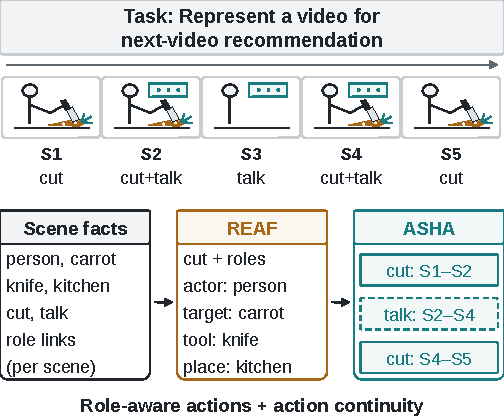
\includegraphics[width=\columnwidth]{figures/hgvrec_motivation.pdf}
  \caption{An illustrative example. REAF encodes who acts on what and
    with which tool; ASHA groups consecutive scenes sharing an action, so
    the two cut segments stay separate.}
  \Description{An illustrative cooking video has five scenes: cut, cut and
    talk, talk, cut and talk, and cut. A person, carrot, knife and kitchen
    provide concrete examples of extracted entities. Three cards show the
    progression from scene facts and extracted role links to role-aware cut
    features and action-segment features. The cut action has a person as
    actor, carrot as target, knife as tool and kitchen as place. Its segments
    span scenes one and two, and four and five. The talk segment spans scenes
    two through four, overlapping both cut segments.}
  \label{fig:hgvrec-motivation}
\end{figure}

%% Queue the wide float here so it can appear on page 2 with the standard
%% two-column output routine. The Methods section refers to it below.
\begin{figure*}[t]
  \centering
  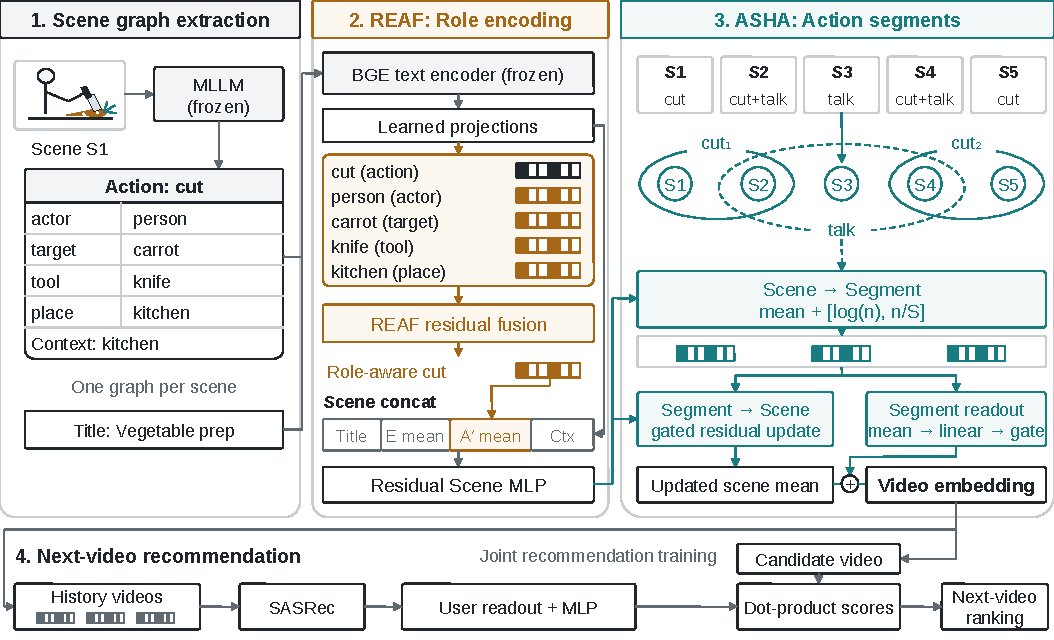
\includegraphics[width=\textwidth]{figures/hgvrec_framework.pdf}
  \caption{Overview of HGVRec on the cooking example. (1) A frozen MLLM turns each
    scene into a graph whose action links entities as actor, target, tool and place.
    (2) REAF fuses the role-linked entity features into the action before pooling a
    scene vector. (3) ASHA groups scenes into contiguous action segments (hyperedges),
    passes messages between scenes and segments, and reads out the video. (4) The same
    encoder embeds history and candidate videos for a SASRec recommender.}
  \Description{Four panels from left to right. Panel 1: a sketched scene of a person
    cutting a carrot is passed to a frozen MLLM, which outputs a small graph: the
    action node cut is linked to person as actor, carrot as target, knife as tool and
    kitchen as place; a context line and the video title are shown below. Panel 2: the
    action vector and four role vectors are stacked and fused into the action; title,
    entity mean, fused action mean and context are concatenated and passed through a
    residual scene MLP. Panel 3: five scene nodes S1 to S5 with three hyperedges drawn
    as bars: cut over S1 and S2, talk over S2 to S4, and a second cut over S4 and S5.
    Boxes describe scene-to-segment aggregation with size features, a gated residual
    segment-to-scene update, and a video readout producing the video embedding.
    Panel 4: history video vectors go through SASRec and a user MLP; a dot product
    with the candidate video embedding gives next-video ranking.}
  \label{fig:hgvrec-framework}
\end{figure*}

% !TeX root = main.tex
\section{Introduction}
\label{sec:introduction}
\begingroup
\setlength{\emergencystretch}{1em}

Video recommendation on Web platforms depends on representations that connect visual content with user preferences.
Multimodal large language models (MLLMs) provide semantic information beyond item metadata: DWYS~\cite{denadai2025dwys} uses generated descriptions as recommendation inputs, while IISAN~\cite{fu2024iisan} adapts multimodal representations through side networks.
Resource constraints can favor compact MLLMs for content extraction.
This raises a representation learning question: how can a recommender make better use of the information that a compact MLLM already extracts?

We investigate explicit structure as a way to improve the recommendation utility of compact MLLM outputs.
A scene may contain entities and actions, yet their separate aggregation leaves participation roles implicit; likewise, aggregating scene vectors without action-level organization leaves continuity implicit.
The opportunity is to expose these relations to the recommender through structured representations of the available observations.

For example, a person may cut vegetables with a knife across several consecutive scenes.
The person, vegetables, and knife play different roles in the same action, while the repeated action links the scenes into a coherent segment.
This suggests contiguous action segments as aggregation units for video representation.
We examine this choice within each video; user interaction histories remain modeled by a sequential recommender.

We introduce HGVRec, a hierarchical framework centered on Action-Segment Hypergraph Aggregation (ASHA).
Building on the general aggregation framework of AllSet~\cite{chien2022allset}, ASHA treats scenes as nodes and maximal contiguous runs sharing a normalized action key as hyperedges.
Scenes with multiple actions can belong to overlapping segments.
Messages pass from scenes to segments and back, with segment extent incorporated into the representations and video readout.
Role-aware Entity--Action Fusion (REAF) supplies ASHA with scene features by fusing entity features into actions according to extracted actor, target, tool, and place assignments.
These explicit memberships and role links make the modeled structure inspectable.

We frame evaluation around structural modeling with a fixed compact MLLM, comparisons with scene sequence and attention encoders, and the use of more capable extractors.
As device chips improve or server AI becomes available, stronger MLLMs may become practical; HGVRec's modular extraction stage allows their recommendation benefits to be investigated within the same framework.
Our contributions and the empirical questions they motivate are:
\begin{itemize}
  \item \textbf{Structured representations from compact MLLMs.}
  We propose a framework that explicitly organizes extracted semantics into role-aware scenes and action segments to improve their utility for recommendation.
  % TODO (A): Verify the gain with the same compact MLLM, visual evidence,
  % recommendation backbone, and evaluation protocol before stating a result.
  \item \textbf{Action segments as aggregation units.}
  We formulate contiguous action grouping as a video representation unit and investigate its utility relative to chronological scene encoding.
  % TODO (B): Add a matched comparison using identical scene features with
  % chronological sequence encoding; report results only after verification.
  \item \textbf{Inspectable relational modeling.}
  ASHA and REAF define explicit scene memberships and role links, supporting structural inspection and comparison with attention-based scene aggregation.
  % TODO (C): Add a matched attention comparison and an actual segment/role
  % example. Structural inspection alone does not establish explanation fidelity.
  \item \textbf{Extension across MLLM capabilities.}
  The framework separates semantic extraction from recommendation learning, enabling evaluation of compact and more capable MLLMs under a common recommendation setup.
  % TODO (D): Add verified comparisons across extractors under the same
  % evaluation protocol; do not infer device latency or memory scalability.
\end{itemize}
\par
\endgroup


% !TeX root = main.tex
% Detailed reading notes and the complete candidate list: related_works/README.md.
\section{Related Works}
\label{sec:related_works}
Video recommendation benefits from modality-specific graph representations, as in MMGCN~\cite{wei2019mmgcn}, MLLM-generated descriptions, as in DWYS~\cite{denadai2025dwys}, and representations from frozen MLLMs fused with item IDs, as in DFF~\cite{sun2026dff}.
Hypergraphs also support recommendation: DHCN~\cite{xia2021dhcn} connects items through sessions, and MHCR~\cite{lyu2025mhcr} combines multiple graph views with hypergraph contrastive learning; HGVRec instead constructs a hypergraph within each video, with scenes as nodes and contiguous action segments as hyperedges.
ASHA follows the node--hyperedge aggregation pattern of HGNN~\cite{feng2019hgnn} and AllSet~\cite{chien2022allset}, using action continuity to define overlapping groups of scenes and incorporating segment extent.
Structured visual representations model entities in semantic roles~\cite{pratt2020gsr} and actions through spatiotemporal scene graphs~\cite{ji2020actiongenome}; REAF uses extracted actor, target, tool, and place assignments to fuse entity features into action representations for recommendation.

% !TeX root = main.tex
% Full-width results table. It is input from main.tex ahead of the Experiments text so that
% the float lands at the top of the page where the results are discussed.
% Rows are generated and checked by
% artifacts/runs/R05_v8_261105/reports/short_paper_numbers.py (--check).
\begin{table*}[t]
  \caption{Recommendation performance (mean$\pm$sample standard deviation over seeds 42, 43, and 44). $\Delta$N and $\Delta$H are relative changes (\%) in NDCG@10 and HR@10 over Title-only. Params counts trainable parameters including the sequential recommender. Bold marks the highest mean.}
  \label{tab:overall-results}
  \centering
  \small
  \setlength{\tabcolsep}{4pt}
  \begin{tabular}{@{}lrcccccccc@{}}
    \toprule
    & & \multicolumn{4}{c}{MicroLens-100K} & \multicolumn{4}{c}{M$^3$L-10M} \\
    \cmidrule(lr){3-6}\cmidrule(l){7-10}
    Method & Params & NDCG@10 & HR@10 & $\Delta$N & $\Delta$H & NDCG@10 & HR@10 & $\Delta$N & $\Delta$H \\
    \midrule
Title-only & 7.62M & .0337$\pm$.0005 & .0642$\pm$.0009 & -- & -- & .1388$\pm$.0019 & .2324$\pm$.0024 & -- & -- \\
Scene Description & 7.62M & .0379$\pm$.0012 & .0726$\pm$.0016 & +12.56 & +13.12 & .1397$\pm$.0017 & .2340$\pm$.0018 & +0.68 & +0.69 \\
Scene Graph & 7.62M & .0351$\pm$.0011 & .0687$\pm$.0019 & +4.25 & +6.97 & .1381$\pm$.0007 & .2324$\pm$.0007 & $-$0.47 & $-$0.03 \\
Scene Graph + ASHA & 8.68M & .0422$\pm$.0010 & .0805$\pm$.0019 & +25.25 & +25.41 & .1423$\pm$.0017 & .2398$\pm$.0019 & +2.50 & +3.16 \\
HGVRec & 8.76M & \textbf{.0434}$\pm$.0004 & \textbf{.0822}$\pm$.0010 & +28.90 & +28.07 & \textbf{.1435}$\pm$.0006 & \textbf{.2405}$\pm$.0006 & +3.38 & +3.45 \\
    \bottomrule
  \end{tabular}
\end{table*}

% !TeX root = main.tex
% Implementation sources: src/validation/{graph_model,scene_segments,model,
% graph_inputs,leave_one_out_recommendation,leave_one_out_execution}.py.
\section{Methods}
\label{sec:methods}

\subsection{Problem Formulation and Overview}
\label{sec:formulation}
Let $\mathcal{V}$ denote the candidate video catalog and $\mathcal{H}_u$ the observed interaction history of user $u$.
HGVRec learns a content representation $\mathbf{z}_v\in\mathbb{R}^{D}$ for each video and a user representation $\mathbf{q}_u\in\mathbb{R}^{D}$ from the history, and ranks candidates for the next interaction by $f(u,v)=\mathbf{q}_u^{\mathsf T}\mathbf{z}_v$; the same video encoder supplies history-item and candidate-item representations.
We observe each video through temporally ordered windows of sampled frames and call a window a \emph{scene}; this does not imply a detected shot or a ground-truth action boundary.
A frozen MLLM produces a scene graph containing entities (name and attributes), action phrases with actor, target, tool, and place assignments, and a scene context (format, medium, and topics).
After structural validation, video $v$ has $S$ valid scenes with original window indices $p_1<\cdots<p_S$.
The video title enters the representation stage as a separate input after visual extraction.
We introduce ASHA first, taking scene vectors $\mathbf{x}_s\in\mathbb{R}^{D}$ as inputs, and then define their construction through REAF (Figure~\ref{fig:hgvrec-framework}).
Throughout, $[\cdot\,;\cdot]$ denotes concatenation and $\sigma$ denotes ReLU.

\subsection{Action-Segment Hypergraph Aggregation (ASHA)}
\label{sec:asha}
A deterministic function $\kappa$ converts an action phrase into a key: it lowercases and tokenizes the phrase, removes participant markers and a fixed set of function words, and normalizes the first remaining token using irregular-form mappings and suffix rules.
This is a lightweight lexical rule that does not merge synonymous actions.
For key $k$, an \emph{action segment} is a maximal run of scenes that contain $k$ and have consecutive original indices ($p_{s+1}=p_s+1$).
A missing window, a scene without $k$, or a later reappearance of $k$ separates segments; singleton segments are retained, and a scene containing several keys belongs to several segments.
A segment thus expresses continuity of an extracted action key rather than a verified continuous real-world event.
The hypergraph has one node per valid scene and the $K$ segments as hyperedges, with fixed incidence $H_{sk}=\mathbb{I}[s\in e_k]$, segment sizes $n_k=\sum_sH_{sk}$, and scene degrees $d_s=\sum_kH_{sk}$.

Following the two-stage aggregation framework of AllSet~\cite{chien2022allset}, ASHA pools each segment and augments it with its extent, updates each scene with the mean of its incident segments, and reads out the video:
\begin{align}
  \mathbf{u}_k &= \sigma\!\left(W_{\mathrm{seg}}\big[\tfrac{1}{n_k}\textstyle\sum_s H_{sk}\mathbf{x}_s;\ \log n_k;\ n_k/S\big]+\mathbf{b}_{\mathrm{seg}}\right), \label{eq:segment}\\
  \mathbf{x}'_s &= \mathbf{x}_s+\alpha\,\mathbb{I}[d_s>0]\,\sigma\!\left(W_{\mathrm{msg}}\big[\mathbf{x}_s;\ \tfrac{1}{d_s}\textstyle\sum_k H_{sk}\mathbf{u}_k\big]+\mathbf{b}_{\mathrm{msg}}\right), \label{eq:scene-update}\\
  \mathbf{z}_v &= \tfrac{1}{S}\textstyle\sum_s\mathbf{x}'_s+\beta\,\mathbb{I}[K>0]\,W_{\mathrm{out}}\tfrac{1}{K}\textstyle\sum_k\mathbf{u}_k. \label{eq:video-readout}
\end{align}
The extent features give the number of member scenes and its fraction of the video's valid scenes.
The scalars $\alpha$ and $\beta$ are trainable and initialized to zero, so ASHA starts as a mean of its input scene vectors; videos without segments keep the scene mean.

\subsection{Role-aware Entity--Action Fusion (REAF)}
\label{sec:reaf}
Let $\phi(\cdot)$ be a frozen text encoder.
We independently project the video title, each entity description, each action phrase, and the scene context into $d$ dimensions with separate learned linear maps of $\phi$, obtaining $\mathbf{t}_v$, $\mathbf{e}$, $\mathbf{a}$, and $\mathbf{c}_s$.
For each action $a$ and role $r$ (actor, target, tool, or place), the role vector $\mathbf{g}_{a,r}$ is the feature of the linked entity, or a learned state $\mathbf{b}_r^{\mathrm{abs}}$ or $\mathbf{b}_r^{\mathrm{unk}}$ when the role is absent or unknown.
With $\mathbf{r}_a$ the concatenation of the four role vectors in this fixed order, REAF updates the action residually:
\begin{equation}
  \widetilde{\mathbf{a}}=\mathbf{a}+\sigma\!\left(W_R[\mathbf{a};\mathbf{r}_a]+\mathbf{b}_R\right).
  \label{eq:reaf}
\end{equation}
The fixed slot order permits different transformations of the same entity feature when it serves different roles; entity features themselves are unchanged.
Let $\overline{\mathbf{e}}_s$ be the mean of projected entity features and $\overline{\mathbf{a}}_s$ the mean of updated action features in scene $s$ (zero if empty).
The scene representation, with $D=4d$, is
\begin{equation}
  \mathbf{x}_s=\mathbf{b}_s+\sigma(W_{\mathrm{scene}}\mathbf{b}_s+\mathbf{b}_{\mathrm{scene}}),\quad
  \mathbf{b}_s=[\mathbf{t}_v;\overline{\mathbf{e}}_s;\overline{\mathbf{a}}_s;\mathbf{c}_s].
  \label{eq:scene-encoder}
\end{equation}
A video with no valid scenes applies the same scene MLP to $[\mathbf{t}_v;\mathbf{0};\mathbf{0};\mathbf{0}]$, so extraction failures do not remove items from the catalog.

\subsection{Sequential Recommendation and Joint Optimization}
\label{sec:objective}
For each prediction event, we retain the most recent $L$ history items, add learned position embeddings to their video vectors, and apply a causally masked SASRec-style Transformer~\cite{kang2018sasrec}.
The hidden state at the last valid position is passed through a two-layer residual user MLP to obtain $\mathbf{q}_u$; the content encoder has no item-ID embedding table.
We train with an in-batch softmax cross-entropy over history--target pairs $(\mathcal{H}_i,y_i)$ using popularity-corrected logits $\mathbf{q}_i^{\mathsf T}\mathbf{z}_{y_j}-\log Q(y_j)$, where $Q$ is the normalized target frequency among training transitions.
Negatives that equal the positive or occur in the input history are masked, and evaluation ranks the uncorrected scores.
All projections, role-state embeddings, REAF, the scene MLP, ASHA, the sequential encoder, and the user MLP are optimized jointly, while the MLLM, the text encoder, and the segment memberships stay fixed.

% !TeX root = main.tex
% Numerical source: artifacts/runs/R05_v8_261105/<dataset>/validation/diagnosis/
% base_description_graph_graph-activity_graph-role-activity/diagnosis.json, via
% R05_v8_261105/reports/paper_evidence.json. Table rows, contrast cells and prose percentages
% are generated and checked by R05_v8_261105/reports/short_paper_numbers.py (--check).
% The stored 10-pair statistical family is preserved even when only four contrasts are shown.
\section{Experiments}
\label{sec:experiments}
We evaluate HGVRec through three questions: \textbf{RQ1} how it compares with title-only, scene-description, and mean-pooled scene-graph representations; \textbf{RQ2} what changes when ASHA is added to the scene-graph encoder; and \textbf{RQ3} what changes when REAF is added to the encoder that already uses ASHA.

\begin{table}[t]
  \caption{NDCG@10 differences ($\times10^{-3}$), relative change (\%) in parentheses, and Bonferroni-corrected 99.5\% paired-bootstrap intervals.}
  \label{tab:contrasts}
  \centering
  \footnotesize
  \setlength{\tabcolsep}{3pt}
  \begin{tabular}{@{}lcc@{}}
    \toprule
    Contrast & MicroLens-100K & M$^3$L-10M \\
    \midrule
    HGVRec $-$ Title-only & 9.74 (28.90) [8.87, 10.59] & 4.69 (3.38) [3.38, 5.95] \\
    HGVRec $-$ Scene Desc. & 5.51 (14.51) [4.71, 6.30] & 3.75 (2.68) [2.46, 5.01] \\
    +ASHA $-$ Scene Graph & 7.08 (20.14) [6.34, 7.80] & 4.13 (2.99) [2.91, 5.34] \\
    HGVRec $-$ +ASHA & 1.23 (2.91) [0.53, 1.92] & 1.22 (0.85) [0.03, 2.42] \\
    \bottomrule
  \end{tabular}
\end{table}

\subsection{Experimental Setup}
\label{sec:experimental-setup}
\paragraph{Datasets and protocol}
We use MicroLens-100K for its micro-video interactions and video content~\cite{ni2025microlens}, and M$^3$L-10M, which adds multimodal movie information, including trailers, to MovieLens-10M~\cite{spillo2026bingewatch}.
For M$^3$L-10M, every rating is treated as an interaction, movies without usable trailer videos are excluded, and the task is predicting the next movie in a rating-event sequence.
Users must have at least five interactions, and we retain their 13 most recent events; the candidate catalog is the union of items in these retained sequences.
This yields 100,000 users, 19,671 items, and 678,355 interactions for MicroLens-100K, and 69,878 users, 8,197 items, and 908,412 interactions for M$^3$L-10M.
The last event of each user is held out for test and the penultimate event for validation.
Validation selects the checkpoint with the highest HR@10; test uses it without refitting, ranking the full catalog after masking all items in the preceding history.

\paragraph{Representation variants}
All variants use the same content-based sequential recommender.
\emph{Title-only} projects the title embedding and applies a residual item MLP.
\emph{Scene Description} combines a projected title with projected scene-description embeddings, applies a residual scene MLP, and averages the scenes.
\emph{Scene Graph} projects title, entity, action, and context features, pools entities and actions separately within each scene, and averages the encoded scenes.
\emph{Scene Graph + ASHA} adds the action-segment module, and \emph{HGVRec} further adds REAF.
The three graph variants share identical extracted graphs, which are valid for 96.04\% and 95.92\% of the scenes in the two datasets; descriptions are a separate extraction.
Scene graphs and descriptions are extracted with Qwen3-VL and embedded with a frozen BGE text encoder.
We train with AdamW (weight decay 0.1, gradient-norm clipping 5.0) and seeds 42, 43, and 44.
% TODO(R05-config): R05 does not archive training.json or the extraction settings. Before
% submission, confirm and state the exact MLLM/BGE checkpoints (was the extractor the 2B
% Instruct model? "compact MLLM" in the Introduction depends on it), window length, frame
% count/resolution, token limits, prompt revisions, d, D, L, Transformer blocks/heads/dropout,
% learning rate, batch size, epoch limit, patience, precision and hardware.
% Do not copy the current config.yaml as R05 settings.

\paragraph{Metrics and statistics}
We report the mean and sample standard deviation of NDCG@10 and HR@10 over the three seeds, with relative changes over Title-only.
For NDCG@10, we average each user's metric over seeds and perform a paired bootstrap over users with 10,000 replicates; Bonferroni correction over all ten pairwise comparisons per dataset at family-wise level $0.05$ yields 99.5\% confidence intervals.
HR@10 is reported descriptively.

\subsection{Results}
\label{sec:overall-results}
\paragraph{Overall performance (RQ1)}
HGVRec achieves the highest mean NDCG@10 and HR@10 among the five variants on both datasets (Table~\ref{tab:overall-results}), with larger relative gains on MicroLens-100K.
Its NDCG@10 intervals against Title-only and Scene Description exclude zero on both datasets (Table~\ref{tab:contrasts}).
Scene Graph alone is below Scene Description on both datasets, indicating that producing graph-formatted outputs and pooling their components is insufficient by itself to reproduce the gains of HGVRec.

\paragraph{Effect of ASHA (RQ2)}
\label{sec:asha-results}
With identical graph inputs, adding ASHA to Scene Graph raises NDCG@10 by 20.14\% and 2.99\%; both corrected confidence intervals are positive, and mean HR@10 also increases.
The comparison adds the complete module (action-segment membership, size-aware segment encoding, scene updates, and segment readout) and its 1.05M trainable parameters.

\paragraph{Effect of REAF (RQ3)}
\label{sec:reaf-results}
Adding REAF to Scene Graph + ASHA increases NDCG@10 by a further 2.91\% and 0.85\% with 83K additional parameters, and both corrected intervals exclude zero.
This supports the incremental benefit of encoding actor, target, tool, and place assignments before pooling actions in the presence of ASHA.

% Working notes, not part of this submission (kept out of the text on purpose):
% matched scene-sequence and attention comparisons, stronger-MLLM extractors, a REAF-only
% variant and parameter-matched controls, grounding/explanation evaluation, and measured
% device latency/memory. Add claims about any of these only together with their results.

% !TeX root = main.tex
\section{Conclusion}
\label{sec:conclusion}
We presented HGVRec, a video representation learning framework that organizes MLLM-extracted semantics through explicit structure: ASHA groups scenes into maximal contiguous action segments and aggregates them through a hypergraph, while REAF encodes entity participation roles within each scene.
On MicroLens-100K and M$^3$L-10M, HGVRec achieves the highest mean NDCG@10 and HR@10 among the five evaluated variants; with shared graph inputs, adding ASHA improves NDCG@10 on both datasets, and adding REAF provides further gains when ASHA is present.

% !TeX root = main.tex
% The ACM bibliography style creates its own References heading.
\bibliographystyle{templates/ACM-Reference-Format}
% Only cited works are printed; the full reading list is in related_works/README.md.
\bibliography{references}


\end{document}
